\documentclass[DIN, pagenumber=false, fontsize=11pt, parskip=half]{scrartcl}

\usepackage{amsmath}
\usepackage{amsfonts}
\usepackage{amssymb}
\usepackage{enumitem}
\usepackage[utf8]{inputenc} % this is needed for umlauts
\usepackage[T1]{fontenc} 
\usepackage{commath}
\usepackage{xcolor}
\usepackage{booktabs}
\usepackage{float}
\usepackage{tikz-timing}
\usepackage{tikz}
\usepackage{multirow}
\usepackage{colortbl}
\usepackage{xstring}
\usepackage{circuitikz}
\usepackage{listings} % needed for the inclusion of source code
\usepackage[final]{pdfpages}
\usepackage{subcaption}

\usetikzlibrary{calc,shapes.multipart,chains,arrows}

\newcommand{\Prb}[1]{P(\text{#1})}
\newcommand{\CPr}[2]{P(\text{#1}|\text{#2})}
\DeclareMathOperator*{\argmax}{arg\,max}
\DeclareMathOperator*{\argmin}{arg\,min}

\title{Pattern Recognition}
\author{Tim Luchterhand, Paul Nykiel, Jonas Strauch (Group P)}

\begin{document}
    \maketitle
    \section{Maximum Likelihood Parameter Estimation}
    \begin{enumerate}
        \item
            \begin{eqnarray*}
                L(p) &=& P({X_1 = n_1}) \land P({X_2 = n_2}) \land P({X_3 = n_3}) \\
                &\stackrel{\text{Variables are independent}}{=}& P({X_1 = n_1}) \cdot P({X_2 = n_2}) \cdot P({X_3 = n_3}) \\
                &\stackrel{\text{Same distribution}}{=}& p \cdot {(1-p)}^{n_1 - 1} \cdot p \cdot {(1-p)}^{n_2 - 1} \cdot p \cdot {(1-p)}^{n_3 - 1} \\
                &\stackrel{\text{Actual values}}{=}& p \cdot {(1-p)}^{1} \cdot p \cdot {(1-p)}^{0} \cdot p \cdot {(1-p)}^{4} \\
                &=& p^3 \cdot {(1-p)}^5
            \end{eqnarray*}
        \item
            First the derivative is calculated:
            \begin{equation*}
                L'(p) = \frac{\text{d}}{\text{d}p} L(p) = 3 p^2 {(1-p)}^5 - 5 p^3 {(1-p)}^4
            \end{equation*}
            Then an extrema is calculated:
            \begin{eqnarray*}
                L'(p) &\stackrel{!}{=}& 0 \\
                \Leftrightarrow 3 p^2 {(1-p)}^5 - 5 p^3 {(1-p)}^4 &=& 0 \\
                \Leftrightarrow 3 p^2 {(1-p)}^5 &=& 5 p^3 {(1-p)}^4 \\
                \stackrel{0 < p < 1}{\Leftrightarrow} 3 (1-p) &=& 5 p \\
                \Leftrightarrow 3 - 3p &=& 5p \\
                \Leftrightarrow 3 &=& 8p \\
                \Leftrightarrow \frac{3}{8} &=& p
            \end{eqnarray*}
        \item
            \lstinputlisting[language=Python]{A1.py}
            \begin{figure}[H]
                \includegraphics[width=\textwidth]{A1.eps}
                \caption{Output of the script}
            \end{figure}
    \end{enumerate}

    \section{Parzen Window (1D)}
    \begin{enumerate}
        \item 
            \begin{enumerate}[label=\alph*)]
                \item By increasing the side length $h$ the width (for the gaussian distributions that is the standard deviation) of the individual kernel functions is increased
                \item For small values of $h$, up to $0.5$, all four data points are in different bins, thus the histogram consists of four equally large bars.
                    For $0.5 < h \leq 2$ the first two data points ($1$ and $1.5$ respectively) belong to one bin, thus the histogram consists of a large bar at $1$ and two bars of half the size at $3$ and $5$. 
                    For $h > 2$ the data point is combined into the bin of the datapoints $1$ and $1.5$, as a result the histogram consists of one large bar, and a small bar which has a third of the height of the last bar. 
                    For values of $h$ larger than $4$, something that can not be visualized on the website, all four data points reside in the same bin, thus the histogram is a single bar.
                \item For small values of $h$ the estimated distribution only consists of a few peaks and thus is not very smooth.
                    For larger values of $h$ the distribution is getting wider and smoother, for $h=2.5$ it looks nearly identical to a single gaussian distribution.
            \end{enumerate}
        \item A suitable value for $h$ should be approximatly $1$, for smaller values the estimated distribution is to "spiky", for larger values the distribution  does not properly model the properties of the distribution.
        \item
            \begin{enumerate}[label=\alph*)]
                \item $ $
                    \begin{figure}[H]
                        \centering
                        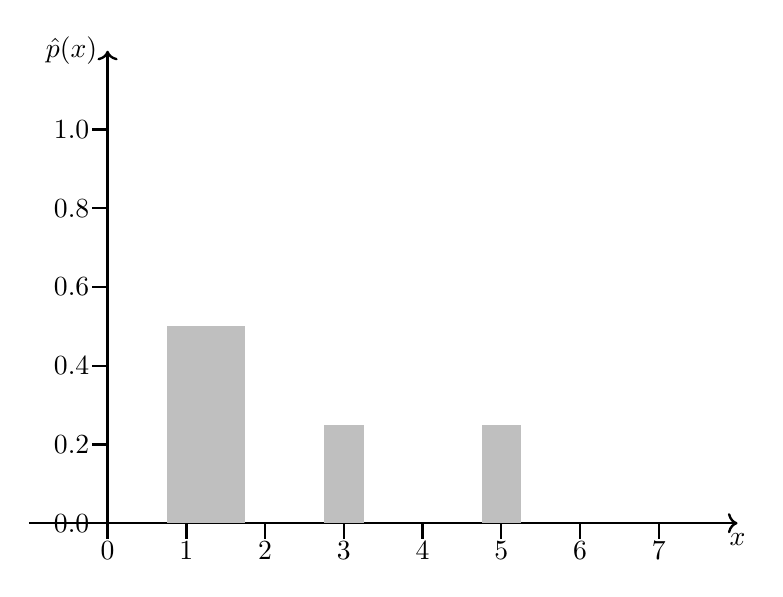
\begin{tikzpicture}
                            \draw[line width=0.3mm, ->] (-1,0) -- (8,0) node[below, pos=1]{$x$};
                            \draw[line width=0.3mm, ->] (0,0) -- (0,6) node[left, pos=1]{$\hat{p}(x)$};
                            \foreach \x in {0,...,7}{
                                \draw[line width=0.3mm] (\x,0) -- (\x,-0.2) node[below, pos=0.5]{$\x$};
                            }
                            \foreach \y in {0,...,4}{
                                \pgfmathtruncatemacro{\label}{\y*2}
                                \draw[line width=0.3mm] (0,\y) -- (-0.2,\y) node[left, pos=0.5]{$0.\label$}; % Hacky hack hack
                            }
                            \draw[line width=0.3mm] (0,5) -- (-0.2,5) node[left, pos=0.5]{$1.0$};

                            \fill[fill=gray!50] (0.75,0) rectangle (1.25,2.5);
                            \fill[fill=gray!50] (1.25,0) rectangle (1.75,2.5);
                            \fill[fill=gray!50] (2.75,0) rectangle (3.25,1.25);
                            \fill[fill=gray!50] (4.75,0) rectangle (5.25,1.25);
                        \end{tikzpicture}
                        \caption{Probability density function estimated using the Parzen window estimate with uniform distributions as a kernel function ($h=0.5$)}
                    \end{figure}
                \item $ $
                    \begin{figure}[H]
                        \centering
                        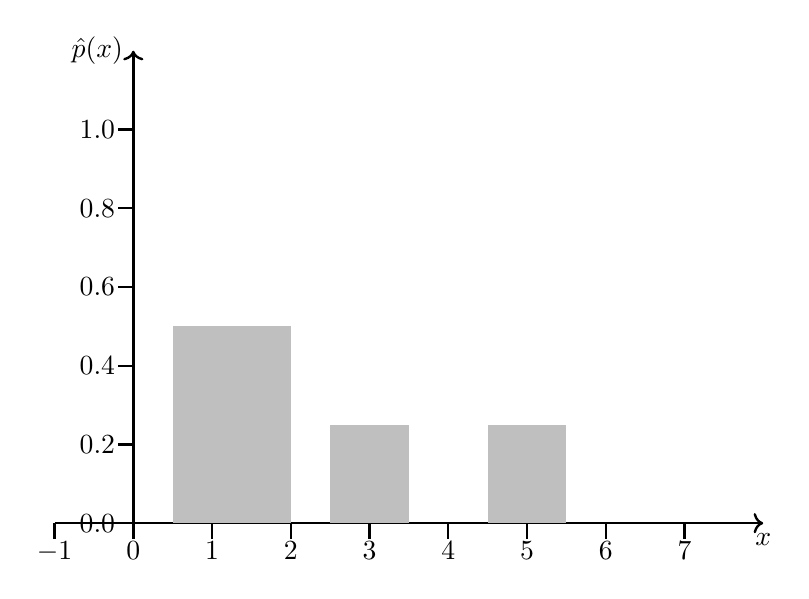
\begin{tikzpicture}
                            \draw[line width=0.3mm, ->] (-1,0) -- (8,0) node[below, pos=1]{$x$};
                            \draw[line width=0.3mm, ->] (0,0) -- (0,6) node[left, pos=1]{$\hat{p}(x)$};
                            \foreach \x in {-1,...,7}{
                                \draw[line width=0.3mm] (\x,0) -- (\x,-0.2) node[below, pos=0.5]{$\x$};
                            }
                            \foreach \y in {0,...,4}{
                                \pgfmathtruncatemacro{\label}{\y*2}
                                \draw[line width=0.3mm] (0,\y) -- (-0.2,\y) node[left, pos=0.5]{$0.\label$}; % Hacky hack hack
                            }
                            \draw[line width=0.3mm] (0,5) -- (-0.2,5) node[left, pos=0.5]{$1.0$};

                            \fill[fill=gray!50] (0.5,0) rectangle (1.5,2.5);
                            \fill[fill=gray!50] (1.0,0) rectangle (2.0,2.5);
                            \fill[fill=gray!50] (2.5,0) rectangle (3.5,1.25);
                            \fill[fill=gray!50] (4.5,0) rectangle (5.5,1.25);
                        \end{tikzpicture}
                        \caption{Probability density function estimated using the Parzen window estimate with uniform distributions as a kernel function ($h=1$)}
                    \end{figure}
                \item $ $
                    \begin{figure}[H]
                        \centering
                        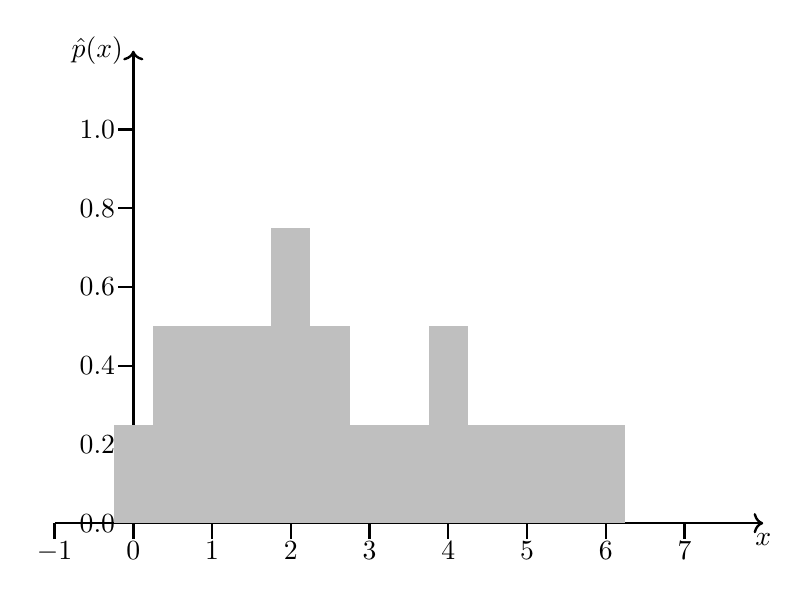
\begin{tikzpicture}
                            \draw[line width=0.3mm, ->] (-1,0) -- (8,0) node[below, pos=1]{$x$};
                            \draw[line width=0.3mm, ->] (0,0) -- (0,6) node[left, pos=1]{$\hat{p}(x)$};
                            \foreach \x in {-1,...,7}{
                                \draw[line width=0.3mm] (\x,0) -- (\x,-0.2) node[below, pos=0.5]{$\x$};
                            }
                            \foreach \y in {0,...,4}{
                                \pgfmathtruncatemacro{\label}{\y*2}
                                \draw[line width=0.3mm] (0,\y) -- (-0.2,\y) node[left, pos=0.5]{$0.\label$}; % Hacky hack hack
                            }
                            \draw[line width=0.3mm] (0,5) -- (-0.2,5) node[left, pos=0.5]{$1.0$};

                            % -0.25-0.25: 1 => 1.25
                            % 0.25-1.75: 2 => 2.5
                            % 1.75-2.25: 3 => 3.75
                            % 2.25-2.75: 2 => 2.5
                            % 2.75-3.75: 1 => 1.25
                            % 3.75-4.25: 2 => 2.5
                            % 4.25-6.25: 1 => 1.25
                            \fill[fill=gray!50] (-0.25,0) rectangle (6.25,1.25);
                            \fill[fill=gray!50] (0.25,0) rectangle (2.75,2.5);
                            \fill[fill=gray!50] (3.75,0) rectangle (4.25,2.5);
                            \fill[fill=gray!50] (1.75,0) rectangle (2.25,3.75);
                        \end{tikzpicture}
                        \caption{Probability density function estimated using the Parzen window estimate with uniform distributions as a kernel function ($h=2.5$)}
                    \end{figure}
            \end{enumerate}
    \end{enumerate}

    \section{Parzen Window (2D)}
    \begin{enumerate}
        \item For the programm see \textit{A3.ipynb}.
            \addtocounter{enumi}{3}
        \item A smooth PDF which still resembles the distribution is achieved with $h=30$.
        \item The value of $h$ depends on the scale of the data points, if all data points are scaled by $f$, $h$ should be scaled by $f$ as well. Thus there can not be a good, fixed, value for $h$ independent of the scale (and thus standard deviation) of the data. 
    \end{enumerate}
\end{document}
